\chapter{Kako sekvenciramo antibiotike?}
\setbookcodestyle


U ovom poglavlju i dalje govorimo o sekvenciranju, ali ćemo proširiti pogled i pokazati različite načine za sekvenciranje peptida. 

\section{Otkriće antibiotika} \label{otkrice}

Pre svega, krenućemo sa biološkim uvodom. Šta su to antibiotici? Sama reč antibiotik znači ,,onaj koji ubija život'', a tačnije, on predstavlja supstancu koja ubija bakterije. Kada ostavimo pomorandžu dugo negde gde je toplo, ona će da razvije čudne osobine kao što je buđ. Šta to znači? Buđ jeste jedna vrsta antibiotika što znači da se antibiotici nalaze u prirodi i da ih proizvode organizmi iz porodice gljiva (npr. buđi) i bakterija. 

Mi ćemo posmatrati antibiotike na molekularnom nivou koji nam govori od čega su oni zapravo izgrađeni. Od svih antibiotika posmatraćemo \textbf{\textit{tirocidin B1}}, antibiotik koji proizvodi bakterija \textit{Bacillus Brevis}. Tirocidin B1 na molekulskom nivou pripada \textit{peptidima}, kratkim niskama aminokiselina, odnosno malim proteinima. Ovo je skok u odnosu na ono što smo do sada posmatrali -- nukleotidne niske nad četvorostrukom azbukom $\Sigma = \{A, C, G, T\}$, odnosno DNK. Za DNK smo govorili da se pojavljuje u svakoj ćeliji svakog živog bića i da je veoma značajna supstanca jer sadrži recept (tačnije, nosi informaciju) za pravilno funkcionisanje i razvoj svakog živog bića. Da bi se svako živo biće pravilno razvijalo, neophodno je da njegove ćelije proizvode (sintetišu) u tačno određeno vreme određene supstance koje se nazivaju \textit{proteini}. DNK nosi informaciju o tome kako treba neki protein da izgleda, od čega treba da se sastoji. Zašto je to bitno? Na primer, kada je dan, neke biljke treba da vrše fotosintezu, a za vršenje fotosinteze treba u samim ćelijama biljaka da se sintetišu određeni proteini.

Proteini su, nakon nukleinskih kiselina, druga značajna grupa molekula koja sa računarske tačke gledišta takođe predstavlja dugačke niske, ali ne nad azbukom od 4 karaktera, nego nad azbukom od 20 karaktera, a svaki karakter predstavlja molekul koji se naziva \textit{aminokiselina}. Kao i nukleinske kiseline, aminokiseline se predstavljaju velikim latiničnim slovima $ \{V, K, L, F, P, W, N, Q, Y, G, A, I, M, D, E, S, T, C, R, H\}$, a pored toga postoje i troslovne oznake $\{Val, Lys, Leu, Phe, Pro, Trp, Asn, Gln, Tyr, Gly, Ala, Ile, Met, Asp, Glu, Ser, Thr, Cys, Arg, His\}$. U prirodi postoji mnogo više od 20 aminokiselina, ali 20 njih najčešće učestvuje u sastav proteina. DNK upravlja time kada će nastati protein u okviru ćelije. Recept za nastajanje svakog proteina je zapisan u DNK. Kako je taj recept zapisan, videćemo u nastavku.

Proteini se još nazivaju i \textit{polipeptidi}. Dužina proteina je obično od 100 aminokiselina do nekoliko hiljada (proteini su kraći od genomske sekvence). Tirocidin B1 je peptid jer se sastoji iz malog broja aminokiselina, svega deset -- $ V,K,L,F,P,W,F,N,Q,Y$. Problem sekvenciranja antibiotika jeste problem određivanja aminokiselina koje ulaze u sastav tog antibiotika. U prethodnom poglavlju smo sekvencirali genom, ali tehnike iz prethodnog poglavlja nećemo moći da koristimo u sekvenciranju tirocidina B1, što će biti objašnjeno u poglavlju \ref{pravljenje}.


\section{Kako bakterije prave antibiotike?} \label{pravljenje}

Pre rešavanja problema sekvenciranja antibiotika, govorićemo o zanimljivoj i kompleksnoj temi, a to je tema -- kako se prave proteini? Već je pomenuto da se u okviru DNK nalazi recept za pravljenje proteina. Sada je vreme da se zapitamo kako je sve to zapisano u DNK pomoću $A, C, G, T$.

Znamo da je DNK dvostruki lanac čiji su krajevi označeni sa 5' i 3' (uvek čitamo lanac od 5' ka 3'). DNK jeste jedna vrsta nukleinskih kiselina koje postoje u ćeliji živih bića. Pored nje, postoje i različite vrste \textbf{ribonukleinskih kiselinina}, odnosno \textbf{RNK}. Ribonukleinske kiseline nisu predstavljene dvostrukim lancem, već jednostrukim. One se sastoje od nukleotida $A, C, G, U$. Umesto timina, kod RNK se pojavljuje nukleotid uracil koji se označava sa $U$. 

DNK se \textbf{\textit{prepisuje}} u RNK. Šta to znači? Da bi nastali proteini, neophodno je da se na osnovu dva lanca od DNK konstruiše RNK molekul. Pošto se RNK molekul sastoji od istih nukleotida kao i DNK, osim timina, onda kažemo da formiranje RNK na osnovu DNK predstavlja jednostavno \textit{prepisivanje} nukleotida iz oba lanca DNK, uz zamenu nukleotida $T$ sa nukleotidom $U$. Drugi naziv za prepisivanje jeste \textit{transkripcija}. Ovo je prvi korak, i dalje nismo došli do aminokiseline, i dalje smo u azbuci nukleotida. RNK predstavlja jedan međukorak između DNK i samog proteina.

Drugi korak jeste \textit{prevođenje}, odnosno \textit{translacija}, prepisanog RNK u proteine. Imamo 4 nukleotida $A, C, G, U$ i treba njih da prevedemo u nisku od 20 mogućih aminokiselina. To znači da mora da postoji neko preslikavanje, nekakav kod koji prevodi neke $k$-grame nukleotida u aminokiseline. Nad azbukom od 4 nukleotida postoji 16 različitih $2$-grama, tj. bigrama. Da li možemo tih 16 bigrama da preslikamo u 20 aminokiselina? Tačnije, da li dva nukleotida možemo da preslikamo u jednu aminokiselinu? Ne možemo, jer moramo za svaku aminokiselinu da znamo koji je bigram označava. Pošto ne možemo to da uradimo sa bigramima, da li možemo sa $3$-gramima? Svih mogućih $3$-grama nad azbukom od 4 nukleotida ima 64. To znači da će svaka od aminokiselina imati svoj kod, a neke od njih će možda imati i više kodova, tj. više trigrama može da ukazuje na jednu aminokiselinu. To je u redu, bitno je da je naša funkcija ,,$na$'', ne mora da bude ,,$1-1$''. Ali kako napraviti funkciju? Ne možemo svojevoljno da dodelimo trigramima određene aminokiseline. Ta funkcija je unapred utvrđena, odnosno, prirodom determinisana i dokazana. U nastavku, koristićemo drugačiji naziv za naše $3$-grame. 
\\
\begin{definicija}
\textbf{Kodon} predstavlja jedan $3$-gram (triplet) nukleotida. \\
\end{definicija}

\noindent Preslikavanje o kojem je do sada bilo reči se naziva \textit{genetski kod} i on je prikazan na slici \ref{slika:genetskiKod}.
\\
\begin{definicija}
\textbf{Genetski kod} predstavlja preslikavanje skupa kodona u skup aminokiselina. \\
\end{definicija}


\begin{figure}[h!]
	\centering
	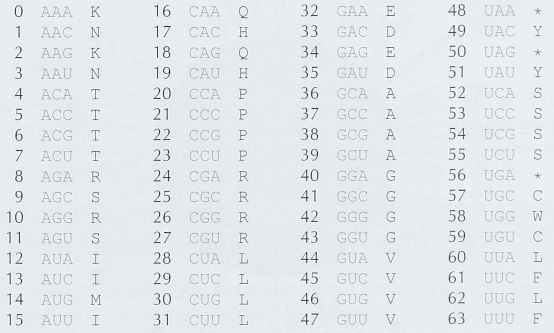
\includegraphics[width=0.8\textwidth]{poglavlja/4/slike/genetskiKod.png}
	\caption{Genetski kod.}
	\label{slika:genetskiKod}
\end{figure} 


Vidimo da se, na primer, kodon $UGG$ preslikava u aminokiselinu $Trp (W)$, dok se više kodona, $CUA, CUC, CUG, CUU, UUA, UUG$, preslikava u jednu aminokiselinu $Lys (L)$. 

Redom, kodone iz RNK preslikavamo u aminokiseline. Ali, kako znamo da je kraj nekog proteina? U genetskom kodu je i tako nešto kodirano. Postoje tzv. \textbf{stop kodoni} koji označavaju da iza njih nema više aminokiselina koje čine taj protein. Ti stop kodoni su $UAA, UAG, UGA$. 

\newpage


Dolazimo do jednog veoma značajnog biološkog aksioma -- \textbf{centralne dogme molekularne biologije}. Ona govori da se transkripcijom na osnovu DNK može dobiti RNK, a translacijom se iz RNK, na osnovu genetskog koda, dobijaju proteini. Ovu teoriju je predstavio Fransis Krik (eng. \textit{Francis Crick}) i prikazana je na slici \ref{slika:centralnaDogma}.
\begin{figure}[h!]
	\centering
	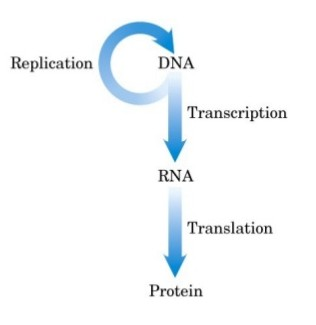
\includegraphics[width=0.5\textwidth]{poglavlja/4/slike/centralnaDog.jpg}
	\caption{Centralna dogma molekularne biologije.}
	\label{slika:centralnaDogma}
\end{figure} 



Ono što želimo da saznamo jeste koje aminokiseline i kojim redom ulaze u sastav našeg malog peptida tirocidina B1. Pošto se on sastoji iz 10 aminokiselina, to znači da ga čine 30 nukleotida u genomu bakterije \textit{Bacillus Brevis} koje će da se prepišu u RNK i da se prevedu iz RNK u tirocidin B1. Hiljade različitih $30$-grama se može prevesti u tirocidin B1 jer se u genetskom kodu različiti kodoni mogu prevesti u istu aminokiselinu. Na slici \ref{slika:30grami} su prikazani neki od takvih $30$-grama. Vidimo da oni nisu previše slični.
\begin{figure}[h!]
	\centering
	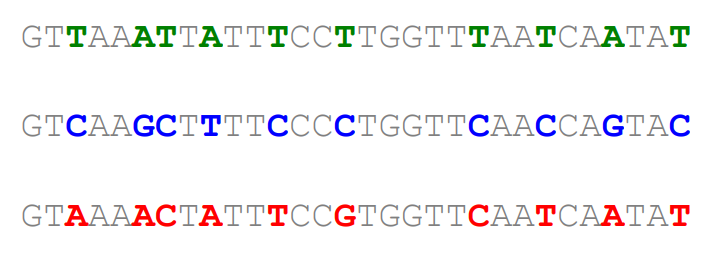
\includegraphics[width=0.8\textwidth]{poglavlja/4/slike/30grami.png}
	\caption{Neki od $30$-grama koji se mogu prevesti u tirocidin B1.}
	\label{slika:30grami}
\end{figure} 
\noindent

 Treba uzeti u obzir da translacija može početi na bilo kojoj poziciji u genomu. To znači da bismo za datu poziciju, ako gledamo $30$-gram, mogli da imamo 6 različitih tzv. \textbf{čitajućih okvira}, tj. 6 varijanti prepisivanja u RNK i onda prevođenja. Tri čitajuća okvira potiču iz tri nukleotida iz jednog kodona iz jednog prevedenog RNK lanca (ako krenemo da čitamo od prvog nukleotida, to je jedan čitajući okvir, iz drugog nukleotida je drugi čitajući okvir, iz trećeg nukleotida je treći čitajući okvir, a ako pročitamo od četvrtog nukleotida, to je već isti čitajući okvir kao prvi jer tu kreće novi kodon), a isto tako za drugi RNK lanac imamo tri čitajuća okvira sa druge strane. 

Naš peptid tirocidin B1 jeste \textit{cikličan}. Tih 10 aminokiselina koje ga čine idu nekim redom, ali su one povezane u krug, tako da imamo ukupno 10 različitih \textbf{linearnih reprezentacija} za tirocidin B1 u zavisnosti od toga koja nam je prva aminokiselina bila u samom receptu DNK. Koju god linearnu reprezentaciju pronađemo, rešili smo problem. 
\\\\
\indent Ne odustajemo od pronalaženja $30$-grama u genomu bakterije \textit{Bacillus Brevis} koji kodira bar jednu linearnu reprezentaciju od svih 10 koje čine tirocidin B1. Pretpostavimo da imamo na raspolaganju veoma moćan računar i neograničeno vreme. Doći ćemo do jednog čudnog rezultata. Nećemo uspeti da pronađemo nijedan $30$-gram u genomu bakterije \textit{Bacillus Brevis} koji kodira bar jednu linearnu reprezentaciju proteina tirocidina B1. Zašto? Stvari se komplikuju. Na ovom primeru je pokazano da centralna dogma ne važi uvek, odnosno ne važi da svaki protein u ćeliji nastaje na osnovu recepta koji je zapisan u DNK. Centralna dogma govori da se proces transkripcije izvršava pod uticajem enzima koji se zove \textit{RNK polimeraza}, a translacija RNK u protein se vrši u ćelijskoj organeli koja se naziva \textit{ribozom}. Postoje neki proteini koji ne nastaju na ovaj način, nego na specijalan način gde obično sekvenciranje genoma ne može da nam pomogne. Moramo da predložimo novi metod kako možemo da pronađemo odgovarajuću sekvencu aminokiselina. 

Edvard Tejtum (eng. \textit{Edward Tatum}), jedan od poznatih američkih genetičara, je 1963. godine inhibirao ribozom bakterije \textit{Bacillus Brevis}. Šta ovo znači? S obzirom da se znalo da se u ribozomu vrši translacija RNK u protein, on je onemogućio da se bilo šta desi u ribozomu, isključio je funkcionisanje te organele u ćeliji i očekivao je da se neće stvoriti nijedan protein, pa ni tirocidin B1. Međutim, suprotno očekivanjima, nastavljena je proizvodnja nekih peptida, uključujući i tirocidine. Ovo je bilo izuzetno iznenađujuće otkriće.

Fric Lipman (eng. \textit{Fritz Lipmann}), američko-nemački biohemičar, je 1969. godine  pokazao da tirocidini spadaju u grupu \textbf{ne-ribozomalnih peptida (NRP-ova)}. To su peptidi za čiju sintezu nisu odgovorni ribozomi i RNK polimeraza već enzimi poznati pod nazivom \textbf{NRP sintetaze}, molekuli koji se takođe nalaze u ćeliji i utiču na različite procese koji se dešavaju u njoj. To znači da se stvaranje tirocidina razlikuje od većeg broja proteina u živim bićima. 
\\\\
\indent Kako izgleda sinteza tirocidina B1 pomoću NRP sintetaze? Postoji veliki broj različitih NRP sintetaza, nije samo jedna odgovorna za stvaranje svih mogućih NRP-ova, nego za svaki ne-ribozomalni peptid postoji odgovarajuća NRP sintetaza. Ona NRP sintetaza koja je odgovorna za stvaranje tirocidina B1 se sastoji od 10 različitih podjedinica koje nazivamo \textit{moduli}. Svaki modul je odgovoran za nadovezivanje jedne aminokiseline na budući molekul tirocidina B1. Svaki od modula privuče jednu aminokiselinu i spoji je sa prethodnom, a poslednji korak jeste cirkularizacija -- spajanje aminokiselina nastalih uz pomoć prvog i poslednjeg modula radi kreiranja cikličnog peptida.

\section{Sekvenciranje antibiotika razbijanjem na komade} \label{razbijanje}

Pošto nam sekvenciranje genomske sekvence i pronalaženje odgovarajuće podniske koja je zadužena za translaciju u aminokiseline odgovarajućeg peptida ne može pomoći u sekvenciranju tirocidina B1 (jer on ne nastaje na osnovu informacije zapisane u DNK), postavljamo pitanje da li postoji način na koji možemo da sekvenciramo antibiotike. Moramo direktno da sekvenciramo peptid. Jedan od načina jeste \textbf{sekvenciranje razbijanjem na komade} i biće predstavljen u ovoj sekciji.
\\\\

\indent U sekvenciranju antibiotika može nam pomoći mašina koja se naziva \textbf{maseni spektrometar} i koju možemo opisati kao skupu molekularnu vagu. Šta on radi? Za početak ćemo da se zapitamo kako možemo da merimo težinu, tačnije masu molekula. 

Pošto se molekuli sastoje od atoma, prvo treba da govorimo o masi pojedinačnog atoma. U atomima postoje protoni, neutroni i elektroni. Protoni i neutroni su približno iste mase, dok su elektroni izuzetno mali i gotovo zanemarljive mase. Zato masu jednog atoma možemo svesti na masu protona, odnosno neutrona koji učestvuju u izgradnji konkretnog atoma koji posmatramo, pa se i masa molekula može izračunati kao suma masa atoma koji ga čine. Maseni spektrometar vraća masu molekula izračunatu u \textbf{Daltonima}. 
\begin{center}
$1 \quad Dalton (Da) \approx masa \quad jednog \quad protona/neutrona$ \\
$Masa \quad molekula \approx suma \quad masa \quad protona/neutrona$
\end{center}

Posmatrajmo masu jedne aminokiseline, recimo glicina. Glicin ima hemijsku formulu $ C_{2}H_{3}ON $. Ugljenik ima masu 12, vodonik ima masu 1, kiseonik 16, a azot 14. Na osnovu ovih masa računamo masu celog molekula glicina.
\begin{center}
$  masa(C_{2}H_{3}ON) = 12*2 + 1*3 + 16*1 + 14*1 \approx 57 Da $
\end{center}

\noindent Simbol  $ \approx $ koristimo jer nam je stvarna masa nešto malo drugačija od celobrojne mase koju dobijamo ovde. Stvarna masa glicina iznosi $ 57.02 Da $. Podrazumevaćemo da je masa celog molekula upravo celobrojna masa koju smo dobili.

Tabela masa svih aminokiselina data je u tabeli \ref{tabela:mase}.

\begin{center}
\begin{table} [h!]
\centering
\caption{Tabela masa 20 aminokiselina poređanih rastuće prema celobrojnim masama.}
\label{tabela:mase}
\begin{tabular}{ |c|c|c|c|c|c|c|c|c|c|c|c|c|c|c|c|c|c|c|c| } 
 \hline
 G & A & S & P & V & T & C & I,L & N &  D & K,Q & E & M & H & F & R & Y & W\\ 
 \hline 
 57 & 71 & 87 & 97 & 99 & 101 & 103 & 113 & 114 & 115 & 128 & 129 & 131 & 137 & 147 & 156 & 163 & 186 \\ 
 \hline
\end{tabular}
\end{table}
\end{center}

Primećujemo da neke aminokiseline imaju iste mase, npr. $I$ i $L$, $K$ i $Q$, pa za 20 aminokiselina imamo 18 celobrojnih masa.

Kada imamo mase aminokiselina, možemo da se zapitamo koja je masa tirocidina B1. Znajući da se tirocidin B1 sastoji iz 10 aminokiselina ovim redom: $ VKLFPWFNQY $, masu računamo koristeći tabelu \ref{tabela:mase}. 

\begin{center}
$  masa(tirocidina \quad B1) = 99+128+113+147+97+186+147+114+128+163 = 1322 $
\end{center}

Vratimo se na maseni spektrometar o kojem smo govorili ranije. Zamislimo da imamo kratak peptid koji se sastoji od samo 4 aminokiseline $NQEL$. Uzorak ovog peptida ubacimo u maseni spektrometar. Šta se u njemu dešava? U njemu se nekim hemijskim procesima, u čije detalje nećemo ulaziti, generišu svi podpeptidi ulaznog peptida. Sa računarske tačke gledišta, maseni spektrometar generiše od zadate niske $NQEL$ sve moguće podniske, podrazumevajući da je ulazni peptid cikličan. Tako se generišu podniske dužine jedan: $N, Q, E, L$, podniske dužine dva: $NQ, QE, EL, LN$ i podniske dužine tri: $NQE$, $QEL$, $ELN$, $LNQ$. Maseni spektrometar za svaki od dobijenih podpeptida može da odredi molekulsku masu. Ono što mi dobijemo kao izlaz iz masenog spektrometra nisu podpeptidi, mi ne znamo koje podpeptide je dobio, niti kojim podpeptidima je prudružena koja masa. Izlaz iz masenog spektrometra jeste samo niz masa! Taj izlazni niz može da sadrži i dva ista broja jer neki podpeptidi mogu da imaju istu masu.

Kako bismo formulisali računarski problem, moramo da definišemo šta je to \textit{teorijski spektar}. 
\begin{definicija} \textbf{Teorijski spektar peptida} predstavlja niz masa svih mogućih podpeptida tog peptida, uključujući nulu kao masu praznog peptida i masu samog peptida.
\end{definicija}

Poznajući sastav peptida, lako možemo da izračunamo teorijski spektar. Suprotan smer je težak, odnosno teško je da na osnovu teorijskog spektra zaključimo kako je izgledao peptid. Upravo ovo jeste problem sekvenciranja ciklopeptida.

\begin{problem}[Problem sekvenciranja ciklopeptida] 
	Rekonstruisati ciklični peptid na osnovu njegovog teorijskog spektra. \\
\end{problem}



\subsection{Sekvenciranje ciklopeptida grubom silom}

Kada dobijemo spektar iz masenog spektrometra, najveća masa će označavati masu celog peptida. Želimo prvo da generišemo sve peptide sa masom jednakom masi celog peptida, zatim da za svaki tako generisan peptid formiramo teorijski spektar i uporedimo ga sa datim spektrom. Algoritam grube sile za problem sekvenciranje ciklopeptida dat je u nastavku. 

\begin{lstlisting}
BFCyclopeptideSequencing(Spectrum)
begin
	// ParentMass(Spectrum) jeste najveca masa u spektru Spectrum
	for every Peptide with Mass(Peptide) equal to ParentMass(Spectrum)
		if Spectrum == CycloSpectrum(Peptide)
			output Peptide
end
\end{lstlisting}

Vidimo da u ovom algoritmu ispitujemo sve kandidate (peptide sa istom masom kao dati peptid). Koliko imamo takvih kandidata? Grafik koji oslikava odgovor na ovo pitanje dat je na slici \ref{slika:kolikoPeptida}.

\begin{figure}[h!]
	\centering
	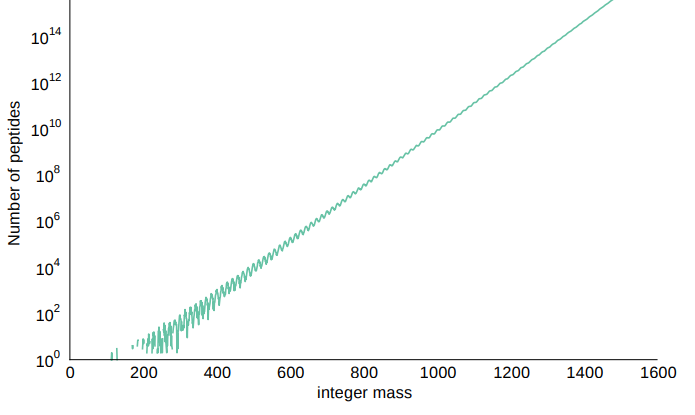
\includegraphics[width=0.7\textwidth]{poglavlja/4/slike/kolikoPeptida.png}
	\caption{Broj peptida sa zadatom masom.}
	\label{slika:kolikoPeptida}
\end{figure} 


Vidimo da je ovaj algoritam grube sile eksponencijalne složenosti. Pod uslovom da imamo dovoljno brz računar, ovako nešto bismo i mogli da izračunamo. Ali, šta bi bili nedostaci ovog algoritma grube sile? Možemo da imamo dva peptida sa istom masom, a da su potpuno različiti. Na primer, peptid $NQEL$ i peptid $TMDH$ imaju masu 484. Kako možemo da isključimo pogrešan peptid? Za oba ova peptida možemo da generišemo teorijski spektar. Ispostavlja se da su njihovi spektri potpuno različiti. Želimo da ovu informaciju iskoristimo u sledećem pristupu rešavanja problema sekvenciranja ciklopeptida. Cilj nam je da ne idemo grubom silom već da ogroman broj kandidata od samog početka odstranimo.
\newpage

\subsection{\textit{Branch-and-Bound} algoritam za sekvenciranje ciklopeptida}

U ovom pristupu postepeno konstruišemo kandidate za rešenja od manjih linearnih peptida za razliku od prethodnog pristupa u kome smo odmah generisali ceo peptid koji postaje kandidat. Na taj način ćemo smanjiti ukupan broj linearnih peptida koje posmatramo. Ovakav pristup se koristi kod \textbf{\textit{Branch-and-Bound} algoritama} koji će biti opisani u nastavku.

Kod \textit{Branch-and-Bound} algoritama u celokupnom prostoru svih mogućih rešenja vršimo nekakva odsecanja. Počnemo od kratkog peptida dužine jedan, pa ga proširimo na sve moguće načine, odnosno, dodamo po jednu aminokiselinu i od toga napravimo sve moguće kandidate dužine dva. To je \textit{branch grana} i predstavljena je na slici \ref{slika:branch}. \textit{Bound grana} bi od postojećih kandidata, nastalih u \textit{branch} granama, isključila neke potencijalne kandidate. \textit{Bound} grana je predstavljena na slici \ref{slika:bound}. Postupak proširivanja i odsecanja ponavljamo sve dok ne dođemo do odgovarajućih vrednosti. Na ovaj način će nam ostati mnogo manje kandidata za rešenja nego u prethodnom pristupu grube sile.

\begin{minipage}{\textwidth}
	\centering
	\begin{minipage}{0.45\textwidth}
		\begin{figure}[H]
			\centering
			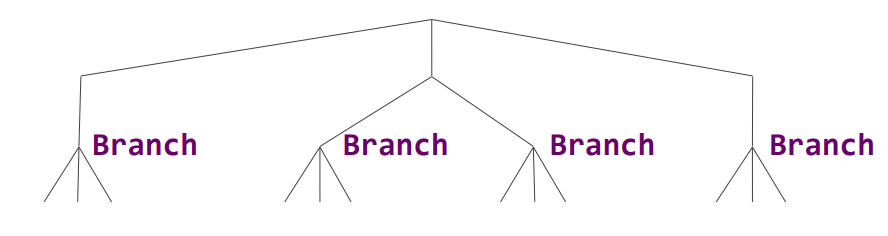
\includegraphics[width=\textwidth]{poglavlja/4/slike/branch.png}
			\caption{\textit{Branch} grane algoritma \textit{Branch-and-Bound}.}
			\label{slika:branch}
		\end{figure} 
	\end{minipage}
	\hfill 
	\begin{minipage}{0.45\textwidth}
		\begin{figure}[H]
			\centering
			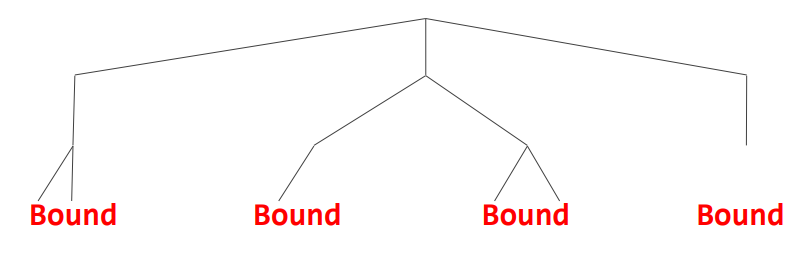
\includegraphics[width=\textwidth]{poglavlja/4/slike/bound.png}
			\caption{\textit{Bound} grane algoritma \textit{Branch-and-Bound}.}
			\label{slika:bound}
		\end{figure} 
	\end{minipage}
	\vspace*{1em}
\end{minipage}

Primenimo ovaj algoritam na konkretan problem. Recimo da nam je dat spektar
\begin{center}
 0 97 97 99 101 103 196 198 198 200 202 295 297 299 299 301 394 396 398 400 400 497.
 \end{center} 
\noindent  Vidimo da se u datom spektru nalaze mase nekih aminokiselina, što nam govori koje aminokiseline ulaze u sastav traženog peptida. Te aminokiseline su $P,V,T,C$ sa masama $97,99, 101, 103$. Ovo znači da možemo da počnemo ne sa svih 20 aminokiselina, nego sa 4 unigrama $P,V,T,C$. Ovo je unapred jedna \textit{bound} grana jer smo 20 aminokiselina sveli na 4 kandidata aminokiselina. Zatim idemo na branch granu, širimo unigrame u sve moguće bigrame: $PA$, $PC$, $PD$,..$PY$, $VA$, $VC$, $VD$,...,$VY$, $TA$, $TC$, $TD$,..., $TY$, $CA$, $CC$, $CD$,..., $CY$. Proširujemo sa svih 20 aminokiselina jer ćemo kasniji videti da ovako zadati spektar jeste čisto teorijski spektar, a maseni spektrometar skoro nikada u praksi ne vraća teorijski spektar već spektar sa nekakvim greškama. Kako možemo da skratimo ovu listu, kako možemo da izvršimo korak \textit{bound} u ovom trenutku? Posmatramo da li postoje odgovarajući bigrami koji se takođe pojavljuju u spektru. Zbog toga uvodimo pojam \textbf{konzistentnosti}.

\begin{definicija}
Za proizvoljan podpeptid $p_{1},..,p_{n}$ kažemo da je \textbf{konzistentan} sa spektrom $S$ ukoliko se svaka masa iz teorijskog spektra podpeptida  $p_{1},..,p_{n}$ nalazi u spektru $S$.
\end{definicija}

Na primer, $PV$ je \textbf{konzistentno} sa spektrom ukoliko se masa od $P$, masa od $V$ i masa od $PV$ nalaze u spektru.

Konzistentnost ćemo koristiti u \textit{bound} koraku, tačnije, izbacićemo sve bigrame koji nisu konzistentni sa spektrom. Tako dobijemo listu konzistentnih bigrama $PV$, $PT$, $PC$, $VP$, $VT$, $VC$, $TP$, $TV$, $CP$, $CV$ koju proširujemo u sve moguće $3$-grame, a zatim svodimo na listu samo konzistentnih $3$-grama. Postupak ponavljamo. Kada dođemo do liste konzistentnih pentagrama $PVCPT$, $PTPVC$, $PTPVC$, $PCVPT$, $VPTPC$, $VCPTP$, $TPVCP$, $TPCVP$, $CPTPV$, $CVPTP$ vidimo da zapravo svi oni pokazuju na jedan isti ciklični peptid.

Pseudokod opisanog algoritma dat je u nastavku.
\begin{lstlisting}
CyclopeptideSequencing(Spectrum)
begin
	Peptides = a set containing only the empty peptide
	while Peptides is non-empty
		// prosirujemo sve peptide u skupu sa svim mogucim aminokiselinama
		Peptides = Expand(Peptides)
		for each Peptide in Peptides
			// ParentMass(Spectrum) jeste najveca masa u spektru
			if Mass(Peptide) = ParentMass(Spectrum)
				if Cyclospectrum(Peptide) = Spectrum
					output Peptide
				remove Peptide from Peptides
			else if Peptide is not consistent with Spectrum
				remove Peptide from Peptides
end
\end{lstlisting}

Podsetimo se da je složenost algoritma grube sile, koji ovde pokušavamo da poboljšamo, eksponencijalna. Ispostavlja se da \textit{Branch-and-Bound} algoritam takođe može biti eksponencijalne složenosti za neke peptide, ali je u praksi veoma brz.



\section{Prilagođavanje sekvenciranja za spektre sa greškama} \label{greskeSpektri}

Spektar koji smo do sada definisali jeste teorijski spektar. Za razliku od njega, spektar koji izlazi iz masenog spektrometra, \textbf{eksperimentalni spektar}, često sadrže greške. O kakvim greškama se govori biće prikazano pomoću slike \ref{slika:ekspSpektar}.

\begin{figure}[h!]
	\centering
	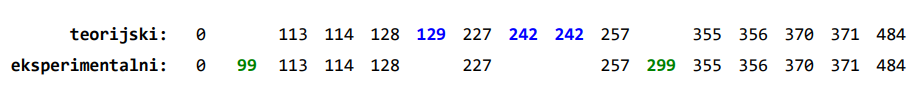
\includegraphics[width=0.9\textwidth]{poglavlja/4/slike/ekspSpektar.png}
	\caption{Primer teorijskog i eksperimentalnog spektra za $NQEL$.}
	\label{slika:ekspSpektar}
\end{figure} 

\textbf{Lažne mase} jesu mase koje su na slici \ref{slika:ekspSpektar} prikazane zelenom bojom. To su mase koje su prisutne u eksperimentalnom spektru, ali nisu prisutne u teorijskom spektru.

\textbf{Nedostajuće mase} jesu mase koje su na slici \ref{slika:ekspSpektar} prikazane plavom bojom. To su mase koje se nalaze u okviru teorijskog spektra, ali ne i u okviru eksperimentalnog spektra.

Zbog pojave ovih otežavajućih okolnosti, tj. grešaka u spektru, neophodan je novi algoritam jer se kod dva predložena algoritma teorijski spektar peptida morao u potpunosti poklapati sa spektrom peptida koji je predstavljao rešenje problema. Sada moramo da olabavimo taj uslov pa uvodimo pojam \textbf{skor peptida}.

\begin{definicija}
\textbf{Skor peptida} pokazuje koliko masa njegov teorijski spektar deli sa eksperimentalnim spektrom.
\end{definicija}

\noindent Tako, za sliku \ref{slika:ekspSpektar}, skor iznosi 11. Želimo da skor bude što veći.

S obzirom da imamo nov način upoređivanja, moramo da unapredimo naš \textit{Branch-and-Bound} algoritam, konkretno korak odsecanja. 

Uzmimo primer golfa. U golfu, kada igrači prođu prvi krug takmičenja, u sledeći krug prolaze dalje samo igrači koji su konkurentni, oni koji imaju šanse da nešto osvoje. To znači da možemo da kažemo da nam je odsecanje takvo da, na primer, prva tri igrača sa najboljim skorom idu dalje, a ukoliko imamo još neke igrače koji imaju isti skor kao poslednji igrač, onda i oni prolaze dalje. Znači, zadržavaju se tri najbolja igrača \textit{,,with ties''}. Ovakav sistem primenjen na \textit{Branch-and-Bound} algoritam prikazan je u sledećem pseudokodu.

\begin{lstlisting}
LeaderboardCyclopeptideSequencing(Spectrum, N)
begin
	Leaderboard = set containing only the empty peptide
	LeaderPeptide = empty peptide
	
	while Leaderboard is non-empty
		// prosirujemo sve elemente koji se nalaze u okviru skupa Leaderboard
		Leaderboard = Expand(Leaderboard)
		for each Peptide in Leaderboard
			// ParentMass(Spectrum) predstavlja najvecu masu u spektru Spectrum
			if Mass(Peptide) == ParentMass(Spectrum)
				if Score(Peptide, Spectrum) > Score(LeaderPeptide, Spectrum)
					LeaderPeptide = Peptide
			else if Mass(Peptide) > ParentMass(Spectrum)
				remove Peptide from Leaderboard
		// odsecamo kandidate iz Leaderboard na osnovu njihovog skora
		Leaderboard = Trim(Leaderboard, Spectrum, N)
		
	output LeaderPeptide
end

Trim(Leaderboard, Spectrum, N, AminoAcid, AminoAcidMass)
begin
	for j=1 to |Leaderboard|
		Peptide = j-th peptide in Leaderboard
		// LinearScore jeste skor nad linearnim spektrom
		LinearScores[j] = LinearScore(Peptide, Spectrum)
		
	sort Leaderboard according to the dec order of scores in LinearScores
	sort LinearScores in dec order
	
	for j=N+1 to |Leaderboard|
		if LinearScores[j] < LinearScores[N]
			remove all peptides starting from the j-th peptide from Leaderboard
			return Leaderboard
			
	return Leaderboard
end
\end{lstlisting}

\noindent \textit{Leaderboard} pristup omogućava da bolje definišemo za esperimentalni spektar kod \textit{Branch-and-Bound} algoritma onu bound fazu kada treba da izbacimo neke kandidate. 

\subsection{Testiranje na spektru tirocidina B1}

U ovom delu razmatraćemo rezultate testiranja na $Spectrum_{10}$, spektru sa 10\% lažnih/nedostajućih masa. 

Kada primenimo \textit{LeaderboardCyclopeptideSequencing} na spektar sa 10\% loših vrednosti, tada zaista dobijemo peptid sa najvišim skorom $ VKLFPWFNQY $  koji odgovara tirocidinu B1. Međutim, ukoliko uzmemo spektar $Spectrum_{25}$ koji ima 25\% lažnih i nedostajućih vrednosti, spektar koji se još više udaljava od teorijskog spektra, onda se peptid sa najvišim skorom $ VKLFPADFNQY $ razlikuje od peptida  $ VKLFPWFNQY $ koji želimo da dobijemo.

Ovo znači da \textit{LeaderboardCyclopeptideSequencing} algoritam radi dobro kada nam je eksperimentalni spektar malo različit od teorijskog.

\section{Od 20 do više od 100 aminokiselina} \label{viseAmino}

U ovoj sekciji biće reči o poboljšanju našeg algoritma uz uvođenje premisa koje postoje u stvarnosti, a koje smo do sada zanemarivali da bismo dali neke početne načine za rešavanje.

Kada smo govorili o proteinima, rekli smo da 20 aminokiselina najčešće učestvuje u njihovoj izgradnji i da su za nas, sa računarske tačke gledišta, proteini niske nad azbukom od 20 karaktera i da postoji još veliki broj aminokiselina nezavisno od izgradnje proteina u ćelijama živih bića. U gentskom kodu postoje kodovi samo za tih 20 aminokiselina, i u tabeli celobrojnih masa aminokiselina postoje mase samo za iste te aminokiseline. S obzirom da u ovom poglavlju razmatramo NRP peptide, peptide koji ne nastaju prema pravilima centralne dogme,  onda ovi peptidi mogu da sadrže i neke nestandardne aminokiseline, one aminokiseline koje se ne nalaze među standardnih 20 aminokiselina. Na primer, tirocidin B sadrži nestandardnu aminokiselinu \textit{Ornitin (Orn)}. Za Ornitin ne postoji nukleotidni triplet u okviru genetskog koda na osnovu koga se ova aminokiselina dobija i ne postoji celobrojna masa u tabeli celobrojnih masa za aminokiseline. S ozbirom na to, možemo da pretpostavimo da bilo koji ceo broj između 57 i 200 (koliko nam iznosi najmanja i najveća masa standardnih aminokiselina) može biti masa neke nestandardne aminokiseline. Ovako nešto može da izgleda kao grubo ograničenje, ali je eksperimentalno potvrđeno da većina masa svih mogućih aminokiselina pripada ovom intervalu.

Spektar u kome nismo ograničeni na tabelu od samo 18 celobrojnih masa, već uzimamo u obzir da bilo koji celi broj između 57 i 200 može da označava neku aminokiselinu, nazivamo \textbf{prošireni spektar}. Kada primenimo Leaderboard algoritam na prošireni spektar sa 10\% lažnih i nedostajućih masa, peptid koji dobijemo $  VKLFPWFN-98-65 $ sadrži neke vrednosti za mase koje ne odgovaraju nijednoj aminokiselini. Pošto Leaderboard algoritam ovde ne daje ispravne vrednosti, moramo da primenimo jedan sasvim novi princip.

\section{Spektralna konvolucija} \label{konvolucija}

Kod algoritma sa proširenim spektrom podrazumeva se da svi celi brojevi između 57 i 200 odgovaraju masama aminokiselina. To znači da razmatramo 144 ili više (znamo da jednoj masi može da odgovara više aminokiselina, a sa druge strane postoje vrednosti kojima ne odgovara nijedna) aminokiselina u koje spadaju i standardne i nestandardne aminokiseline. Želimo da smanjimo broj aminokiselina koje razmatramo. 

Posmatrajmo eksperimentalni spektar za $ NQEL $
\begin{center}
0 99 113 114 128 227 257 299 355 356 370 371 484.
\end{center}
\noindent Mi znamo da je $ Mass(E) = 129 $ i vidimo da u spektru ne postoji ta vrednost. Sa druge strane, u spektru postoji $ Mass(QE) = 257 $ i $ Mass(Q) = 128 $. Razlika ove dve mase daje vrednost $129$. Ova vrednost već deluje kao dobra vrednost za nedostajuću masu. U spektru postoji još ovakvih slučajeva. Recimo, $ Mass(ELN) - Mass(LN) = 356 - 227 = 129 $ i $ Mass(NQEL) - Mass(LNQ) = 484 - 355 = 129 $. Obe ove razlike ukazuju na masu od $E$ koja nedostaje.

Uvodimo tabelu koja se naziva \textbf{spektralna konvolucija}.
\begin{definicija}
\textbf{Spektralna konvolucija} je tabela koja pokazuje apsolutnu vrednost razlike između svake dve mase u spektru.
\end{definicija}

Primer spektralne konvolucije za spektar čije su lažne vrednosti označene sa ,,false'' prikazan je na slici \ref{slika:spektralnaKonvolucija}.

\begin{figure}[h!]
	\centering
	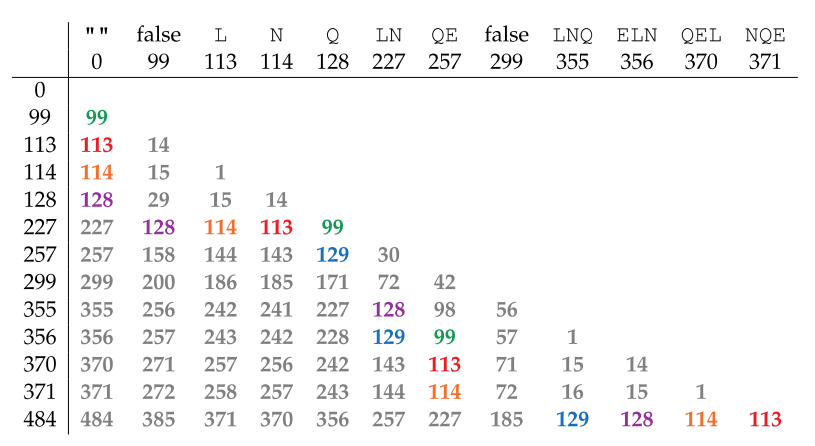
\includegraphics[width=0.9\textwidth]{poglavlja/4/slike/spektralnaKonvolucija.png}
	\caption{Primer spektralne konvolucije.}
	\label{slika:spektralnaKonvolucija}
\end{figure}

\noindent Na preseku svake vrste i kolone u spektralnoj konvoluciji upisana je apsolutna vrednost razlike celobrojnih masa. Kako iskoristiti spektralnu konvoluciju? Tražimo vrednosti razlika koje se pojavljuju najveći broj puta, a da se nalaze između 57 i 200. Obojene vrednosti na slici \ref{slika:spektralnaKonvolucija} se pojavljuju veći broj puta. To su vrednosti 99, 113, 114, 128 i 129. Ove vrednosti odgovaraju masama aminokiselina, redom, $V, L, N, Q, E $. Od 5 najčešćih aminokiselina u konvoluciji 4 čine peptid $NQEL$.

Kako bi izgledao unapređeni algoritam za sekvenciranje ciklopeptida ukoliko uzmemo u obzir i nestandardne aminokiseline, odnosno proširenu tabelu celobrojnih masa aminokiselina? Pseudokod je dat u nastavku.
\begin{lstlisting}
ConvolutionCyclopeptideSequencing(Spectrum, N, M)
begin
	Formirati spektralnu konvoluciju spektra Spectrum.
	Uzeti M najcescih elemenata u konvoluciji (izmedju 57 i 200).
	Primeniti LeaderboardCyclopeptideSequencing, formirajuci peptide samo na osnovu ovih M celih brojeva.
end
\end{lstlisting}

Algoritam  \textit{ConvolutionCyclopeptideSequencing} daje tačan rezultat i za spektre sa šumom od 10\% i za spektre sa šumom od 25\%, što pokazuje da je spektralna konvolucija odgovorila na sve izazove koji su postavljeni.

\section{Spektri u realnosti} \label{realnost}

Kao što znamo, realnost je obično drugačija. Neke poteškoće iz realnosti smo zanemarivali. Koje?
\begin{itemize}
	\item $Spectrum_{25}$ je mnogo manje šumovit nego spektri dobijeni u praksi iz masenog spektrometra.
	
	\item Maseni spektrometar ne meri jednostavno fragmente podpeptida, već su postupci merenja mnogo komplikovaniji. Najpre se zaista vrši razbijanje datog peptida na fragmente. Zatim se oni sortiraju, korišćenjem elektromagnetnog polja, prema svojoj masi. Ono što maseni spektrometar meri jeste zapravo \textbf{odnos mase i naelektrisanja} za svaki fragment (znači nije baš masa) i određuje \textbf{intenzitet} (kao broj jona) u svakom odnosu mase i naelektrisanja. Šta to znači? To znači da kao izlaz iz masenog spektrometra ne dobijamo eksperimentalni spektar koji smo do sada imali prilike da vidimo, nego grafik intenziteta prema odnosu mase i naelektrisanja sa vrhovima na određenim mestima. Primer ovakvog grafika dat je na slici \ref{slika:intenzitet}.
	\begin{figure}[h!]
	\centering
	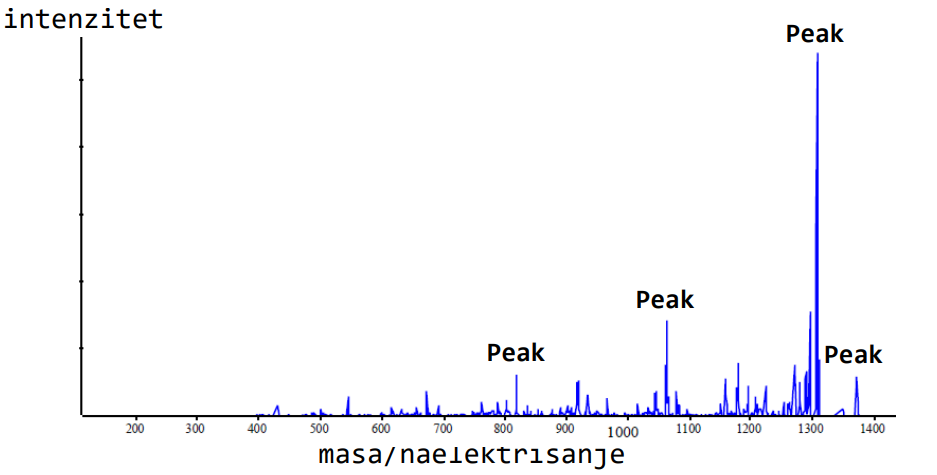
\includegraphics[width=0.9\textwidth]{poglavlja/4/slike/intenzitet.png}
	\caption{Primer grafika intenziteta prema odnosu mase i naelektrisanja.}
	\label{slika:intenzitet}
\end{figure}
	Na osnovu vrhova na grafiku, određivaćemo sam sastav peptida. Ovaj grafik se naziva \textbf{realni spektar}. Rekonstrukcija peptida na osnovu realnog spektra biće obrađena u poglavlju 11.
	
\end{itemize}

\newpage
\section{Zadaci sa vežbi}
\setexamplecodestyle

U nastavku će biti predstavljeni zadaci sa vežbi na kursu rađeni u programskom jeziku Python.

\subsection{Linear Spectrum}

\lstinputlisting[language=Python]{poglavlja/4/kodovi/LinearSpectrum.py}

\subsection{Cyclic Spectrum}

\lstinputlisting[language=Python]{poglavlja/4/kodovi/CyclicSpectrum.py}

\subsection{Cyclopeptide Sequencing}

\lstinputlisting[language=Python]{poglavlja/4/kodovi/CyclopeptideSequencing.py}

\subsection{Leaderboard Cyclopeptide Sequencing}

\lstinputlisting[language=Python]{poglavlja/4/kodovi/LeaderboardCyclopeptideSequencing.py}